\section*{NAIL062 V\&P Logika: 4. sada příkladů -- Tablo metoda}
% po 4. přednášce



\subsection*{Cíle výuky:} Po absolvování cvičení student

    \begin{itemize}\setlength{\itemsep}{0pt}
        \item zná potřebné pojmy z tablo metody (položka, tablo, tablo důkaz/zamítnutí, dokončená/sporná větev, kanonický model), umí je formálně definovat, uvést příklady
        \item zná všechna atomická tabla, a umí vytvořit vhodná atomická tabla pro libovolnou logickou spojku
        \item umí sestrojit dokončené tablo pro danou položku z dané (i nekonečné) teorie
        \item umí popsat kanonický model pro danou dokončenou bezespornou větev tabla
        \item umí aplikovat tablo metodu k řešení daného problému (slovní úlohy, aj.)
        \item zná větu o kompaktnosti, umí ji aplikovat
    \end{itemize}
    

\section*{Příklady na cvičení}


\begin{problem}
    
    Aladin našel v jeskyni dvě truhly, A a B. Ví, že každá truhla obsahuje buď poklad, nebo smrtonosnou past.
    \begin{itemize}
    \item Na truhle A je nápis: {\it ``Alespoň jedna z těchto dvou truhel obsahuje poklad.''}
    \item Na truhle B je nápis: {\it ``V truhle A je smrtonosná past.''}
    \end{itemize}
    Aladin ví, že buď jsou oba nápisy pravdivé, nebo jsou oba lživé.
    \begin{enumerate}[(a)]
        \item Vyjádřete Aladinovy informace jako teorii $T$ nad vhodně zvolenou množinou výrokových proměnných $\mathbb P$. (Vysvětlete význam jednotlivých výrokových proměnných v $\mathbb P$.)
        \item Pokuste se sestrojit tablo důkazy, z teorie $T$, výroků o významu ``Poklad je v truhle A'' a ``Poklad je v truhle B''.
        \item Je-li některé z těchto dokončených tabel bezesporné, sestrojte kanonický model pro některou z jeho bezesporných větví.
        \item Jaký závěr z toho můžeme učinit?
    \end{enumerate}

    \begin{solution}
        \begin{enumerate}[(a)]
            \item Z kontextu poznáme, že `buď, \dots nebo' je exkluzivní (truhla nemůže obsahovat zároveň poklad i smrtonosnou past). Zvolíme jazyk $\mathbb P=\{a,b\}$, kde $a$ znamená `truhla A obsahuje poklad', podobně pro $b$. Nápisy na truhlách formalizujeme jako výroky $a\lor b,\neg a$. Teorie $T$ vyjadřuje, že jsou oba pravdivé nebo oba lživé:
            $$
            T=\{((a\lor b)\land \neg a)\lor(\neg (a\lor b)\land \neg\neg a)\}
            $$
            (Alternativně bychom mohli formalizovat jako $T=\{(a\lor b)\liff \neg a\}$, tj. nahlédnout, že ``oba pravdivé nebo oba lživé'' znamená ekvivalenci. Tabla by byla trochu menší, ale jinak podobná---vyzkoušejte si!)
            \item Tabla budou mít v kořeni položky $\mathrm{F}a$ resp. $\mathrm{F}b$ (dokazujeme `sporem'):
            %\begin{multicols}{2}
                \begin{center}
                    \begin{forest}
                        [$\mathrm{F}a$
                            [$\mathrm{T}((a\lor b)\land \neg a)\lor(\neg (a\lor b)\land \neg\neg a)$
                                [$\mathrm{T}(a\lor b)\land \neg a$
                                    [$\mathrm{T}(a\lor b)$
                                        [$\mathrm{T}\neg a$
                                            [$\mathrm{F}a$
                                                [$\mathrm{T}a$, tikz={\node[fit to=tree,label=below:$\otimes$] {};}]
                                                [$\mathrm{T}b$, tikz={\node[fit to=tree,label=below:$\checkmark$] {};}]
                                            ]
                                        ]
                                    ]                            
                                ]
                                [$\mathrm{T}\neg (a\lor b)\land \neg\neg a$
                                    [$\mathrm{T}\neg (a\lor b)$
                                        [$\mathrm{T}\neg\neg a$
                                            [$\mathrm{F}\neg a$
                                                [$\mathrm{T}a$, tikz={\node[fit to=tree,label=below:$\otimes$] {};}]
                                            ]
                                        ]
                                    ]
                                ]
                            ]                        
                        ]            
                    \end{forest}
                \end{center}                

                \begin{center}
                    \begin{forest}
                        [$\mathrm{F}b$
                            [$\mathrm{T}((a\lor b)\land \neg a)\lor(\neg (a\lor b)\land \neg\neg a)$
                                [$\mathrm{T}(a\lor b)\land \neg a$
                                    [$\mathrm{T}(a\lor b)$
                                        [$\mathrm{T}\neg a$
                                            [$\mathrm{T}a$
                                                [$\mathrm{F}a$, tikz={\node[fit to=tree,label=below:$\otimes$] {};}]
                                            ]
                                            [$\mathrm{T}b$, tikz={\node[fit to=tree,label=below:$\otimes$] {};}]
                                        ]
                                    ]                            
                                ]
                                [$\mathrm{T}\neg (a\lor b)\land \neg\neg a$
                                    [$\mathrm{T}\neg (a\lor b)$
                                        [$\mathrm{T}\neg\neg a$
                                            [$\mathrm{F}a\lor b$
                                                [$\mathrm{F}a$
                                                    [$\mathrm{F}b$
                                                        [$\mathrm{F}\neg a$
                                                            [$\mathrm{T}a$, tikz={\node[fit to=tree,label=below:$\otimes$] {};}]
                                                        ]
                                                    ]
                                                ]
                                            ]
                                        ]
                                    ]
                                ]
                            ]                        
                        ]            
                    \end{forest}
                \end{center}
            %\end{multicols}
            \item První tablo je dokončené, ale bezesporné. Bezesporná větev obsahuje položky $\mathrm{F}a$, $\mathrm{T}b$, kanonický model pro tuto větev je $v=(0,1)$. Je to model teorie $T$ (všechny jeho větve jsou sporné), ve kterém v truhle A není poklad, tedy protipříklad k tvrzení, že v truhle A je poklad.
            \item Druhé tablo je sporné, jde tedy o tablo důkaz a víme, že v truhle B je poklad.
        \end{enumerate}

    \end{solution}

\end{problem}


\begin{problem}

    Uvažme nekonečnou výrokovou teorii (a) $T=\{p_{i+1} \to p_i\mid i\in \mathbb{N}\}$ (b) $T=\{p_i \to p_{i+1}\mid i\in \mathbb{N}\}$. Pomocí tablo metody najděte všechny modely $T$. Je každý model $T$ kanonickým modelem pro některou z větví tohoto tabla? %(Můžete se pokusit sestrojit také \emph{systematické} tablo.)

    \begin{solution}

        Sestrojíme tablo z teorie $T$, do kořene dáme položku $\mathrm{T}\alpha_0$, kde $\alpha_0$ je první axiom $T$. Ukážeme jen začátek konstrukce, potřebujete-li, zkonstruujte více.

        Nejprve vyřešme (a):
        
        \begin{center}
            \begin{forest}
                [$\mathrm{T}p_1\to p_0$ 
                    [$\mathrm{F}p_1$
                        [$\mathrm{T}p_2\to p_1$ 
                            [$\mathrm{F}p_2$
                                [$\mathrm{T}p_3\to p_2$ 
                                    [$\mathrm{F}p_3$, tikz={\node[fit to=tree,label=below:$\vdots$] {};}]
                                    [$\mathrm{T}p_2$, tikz={\node[fit to=tree,label=below:$\otimes$] {};}]              
                                ] 
                            ]
                            [$\mathrm{T}p_1$, tikz={\node[fit to=tree,label=below:$\otimes$] {};}]              
                        ]
                    ]
                    [$\mathrm{T}p_0$
                        [$\mathrm{T}p_2\to p_1$ 
                            [$\mathrm{F}p_2$
                                [$\mathrm{T}p_3\to p_2$ 
                                    [$\mathrm{F}p_3$, tikz={\node[fit to=tree,label=below:$\vdots$] {};}]
                                    [$\mathrm{T}p_2$, tikz={\node[fit to=tree,label=below:$\otimes$] {};}]         
                                ]
                            ]
                            [$\mathrm{T}p_1$
                                [$\mathrm{T}p_3\to p_2$ 
                                    [$\mathrm{F}p_3$, tikz={\node[fit to=tree,label=below:$\vdots$] {};}]
                                    [$\mathrm{T}p_2$, tikz={\node[fit to=tree,label=below:$\vdots$] {};}]         
                                ]
                            ]              
                        ]
                    ]
                ]
            \end{forest}
        \end{center}
        Každý model $T$ se shoduje s některou (bezespornou) větví tohoto (dokončeného) tabla. (Zde dokonce platí, že každý model $T$ je \emph{kanonickým} modelem pro některou z větví. Obecně to ale neplatí.) Modely jsou: $\M(T)=\{v_{<k}\mid k\in\mathbb N\}\cup\{v_\text{all}\}$ kde $v_\text{all}(p_i)=1$ pro všechna $i\in\mathbb N$, a
        $$
        v_{<k}(p_i)=\begin{cases}
            1 & \text{ if }i<k,\\
            0 & \text{ if }i\geq k.            
        \end{cases}
        $$
        
        Nyní (b):

        \begin{center}
            \begin{forest}
                [$\mathrm{T}p_0\to p_1$ 
                    [$\mathrm{F}p_0$
                        [$\mathrm{T}p_1\to p_2$ 
                            [$\mathrm{F}p_1$
                                [$\mathrm{T}p_2\to p_3$ 
                                    [$\mathrm{F}p_2$, tikz={\node[fit to=tree,label=below:$\vdots$] {};}]
                                    [$\mathrm{T}p_3$, tikz={\node[fit to=tree,label=below:$\vdots$] {};}]              
                                ] 
                            ]
                            [$\mathrm{T}p_2$
                                [$\mathrm{T}p_2\to p_3$ 
                                    [$\mathrm{F}p_2$, tikz={\node[fit to=tree,label=below:$\otimes$] {};}]
                                    [$\mathrm{T}p_3$, tikz={\node[fit to=tree,label=below:$\vdots$] {};}]         
                                ]
                            ]              
                        ]
                    ]
                    [$\mathrm{T}p_1$
                        [$\mathrm{T}p_1\to p_2$ 
                            [$\mathrm{F}p_1$, tikz={\node[fit to=tree,label=below:$\otimes$] {};}]         
                            [$\mathrm{T}p_2$
                                [$\mathrm{T}p_2\to p_3$ 
                                    [$\mathrm{F}p_2$, tikz={\node[fit to=tree,label=below:$\otimes$] {};}]
                                    [$\mathrm{T}p_3$, tikz={\node[fit to=tree,label=below:$\vdots$] {};}]         
                                ]
                            ]              
                        ]
                    ]
                ]
            \end{forest}
        \end{center}

        Opět není těžké nahlédnout, že každý model se shoduje s některou z větví. Máme $\M(T)=\{v_\text{none}\}\cap\{v_{\geq k}\mid k\in\mathbb N\}$ kde $v_\text{none}(p_i)=0$ pro všechna $i\in\mathbb N$, a
        $$
        v_{\geq k}(p_i)=\begin{cases}
            0 & \text{ if }i<k,\\
            1 & \text{ if }i\geq k.            
        \end{cases}
        $$
                    
    \end{solution}

\end{problem}


\begin{problem}

    Navrhněte vhodná atomická tabla pro logickou spojku $\oplus$ (XOR) a ukažte, že souhlasí-li model s kořenem vašich atomických tabel, souhlasí i s některou větví.

    \begin{solution}

        Potřebujeme dvě atomická tabla, pro položky tvaru $\mathrm{T}\varphi\oplus\psi$ a $\mathrm{F}\varphi\oplus\psi$. Mohou vypadat například následovně, podmínku si ověřte sami (snadno sémanticky):

        \begin{multicols}{2}

            \centering
            \begin{forest}
                [$\mathrm{T}\varphi\oplus\psi$
                    [$\mathrm{T}\varphi$
                        [$\mathrm{F}\psi$]
                    ]
                    [$\mathrm{F}\varphi$
                        [$\mathrm{T}\psi$]
                    ]                        
                ]            
            \end{forest}

            \begin{forest}
                [$\mathrm{F}\varphi\oplus\psi$
                    [$\mathrm{T}\varphi$
                        [$\mathrm{T}\psi$]
                    ]
                    [$\mathrm{F}\varphi$
                        [$\mathrm{F}\psi$]
                    ]                        
                ]            
            \end{forest}

        \end{multicols}
                    
    \end{solution}
        
\end{problem}


\begin{problem}
    Pomocí věty o kompaktnosti ukažte, že každé spočetné částečné uspořádání lze rozšířit na úplné (lineární) uspořádání.

    \begin{solution}

        Pro konečná částečná uspořádání se dokáže snadno (podobně jako topologické uspořádání acyklického orientovaného grafu). 
        
        Mějme spočetně nekonečnou částečně uspořádanou množinu $\langle X;\leq^X\rangle$. Sestrojíme výrokovou teorii $T$ takovou, aby její modely popisovaly lineární uspořádání na $X$ rozšiřující $\leq^X$. Bude sestávat z následujících množin výroků:
        \begin{itemize}
            \item $p_{xx}$ pro všechna $x\in X$ \hfill (reflexivita)
            \item $p_{xy}\limplies\neg p_{yx}$ pro všechna $x\neq y\in X$ \hfill (antisymetrie)
            \item $p_{xy}\land p_{yz}\limplies p_{xz}$ pro všechna $x,y,z\in X$ \hfill (tranzitivita)
            \item $p_{xy}\lor p_{yx}$ pro všechna $x,y\in X$ \hfill (linearita)
            \item $p_{xy}$ pro všechna $x,y$ taková, že $x\leq^X y$\hfill (jde o rozšíření $\leq^X$)
        \end{itemize}
        (Reflexivitu lze vynechat, plyne už z toho, že jde o rozšíření reflexivní relace $\leq^X$.)

        Dokazujme: $\langle X;\leq^X\rangle$ má lineární rozšíření, právě když $T$ má model, to je z věty o kompaktnosti právě když každá konečná část $T$ má model. Vezměme libovolnou konečnou $T'\subseteq T$. Stačí tedy ukázat, že $T'$ má model. Označme jako $X'$ množinu všech $x\in X$, \emph{o kterých mluví $T'$}, tj.:
        $$
        X'=\{x\in X\mid p_{xy}\in\mathrm{Var}(T')\text{ nebo }p_{yx}\in\mathrm{Var}(T')\text{ pro nějaké }y\in X\}
        $$
        Protože $T'$ je konečná, je i $X'$ konečná množina. Buď $\leq^{X'}$ restrikce $\leq^X$ na množinu $X'$, neboli $\leq^{X'}\,=\,\leq^X \mathbin{\cap}\, (X'\times X')$. Toto konečné částečné uspořádání lze rozšířit na lineární uspořádání $\leq^{X'}_L$, což nám dává model teorie $T'$ (kde $v(p_{xy})=1$ právě když $x\leq^{X'}_L y$).
        
    \end{solution}
    
\end{problem}
        
        
\section*{Další příklady k procvičení}


\begin{problem}

    Adam, Barbora a Cyril jsou vyslýcháni, při výslechu bylo zjištěno následující:
    \begin{enumerate}[(i)]\it
        \item Alespoň jeden z vyslýchaných říká pravdu a alespoň jeden lže.
        \item Adam říká: \emph{``Barbora nebo Cyril lžou''}
        \item Barbora říká: \emph{``Cyril lže''}
        \item Cyril říká: \emph{``Adam nebo Barbora lžou''}
    \end{enumerate}
    \begin{enumerate}[(a)]
        \item Zapište tvrzení $(i)$ až $(iv)$ jako výroky $\varphi_1$ až $\varphi_4$ nad množinou prvovýroků $\mathbb{P}=\{a,b,c\}$, přičemž $a,b,c$ znamená (po řadě), že {\it ``Adam/Barbora/Cyril říká pravdu''}.
        \item Pomocí tablo metody dokažte, že z teorie $T = \{\varphi_1, \dots, \varphi_4\}$ plyne, že Adam říká pravdu.
        \item Je teorie $T$ ekvivalentní s teorií $T' = \{\varphi_2, \varphi_3, \varphi_4\}$? Zdůvodněte.    
    \end{enumerate}
    
\end{problem}
        

\begin{problem}

    Pomocí tablo metody dokažte, že následující výroky jsou tautologie:
    \begin{enumerate}[(a)]
        \item $(p\to (q \to q))$
        \item $p \leftrightarrow \neg \neg  p$
        \item $\neg (p \vee q) \leftrightarrow (\neg p \wedge \neg q)$
        \item $(p \to q) \leftrightarrow (\neg q \to \neg p)$    
    \end{enumerate}

\end{problem} 
   

\begin{problem}
    
    Pomocí tablo metody dokažte nebo najděte protipříklad ve formě \emph{kanonického} modelu pro bezespornou větev.
    \begin{enumerate}[(a)]
        \item $\{ \neg q,\ p \vee q\} \models p$
        \item $\{ q \to p,\ r \to q,\ (r \to p) \to s\} \models s$
        \item $\{ p \to r,\ p \vee q,\ \neg s \to \neg q\} \models r \to s$
    \end{enumerate}

\end{problem}


\begin{problem}

    Pomocí tablo metody určete všechny modely následujících teorií:
    \begin{enumerate}[(a)]
        \item $\{(\neg p \vee q) \to (\neg q \wedge r)\}$
        \item $\{\neg q \to (\neg p \vee q),\ \neg p \to q,\ r \to q\}$
        \item $\{ q \to p,\ r \to q,\ (r \to p) \to s\}$
    \end{enumerate}

\end{problem}


\begin{problem} 
    Navrhněte vhodná atomická tabla a ukažte, že souhlasí-li model s kořenem vašich atomických tabel, souhlasí i s některou větví:
    \begin{itemize}
        \item pro Peirceovu spojku $\downarrow$ (NOR),
        \item pro Shefferovu spojku $\uparrow$ (NAND),
        \item pro $\oplus$ (XOR),
        \item pro ternární operátor ``if p then q else r'' (IFTE).
    \end{itemize}  
    
\end{problem}


\begin{problem}

    \emph{Half-adder circuit} je logický obvod se dvěma vstupními bity (bit 1, bit 2) a dvěma výstupními bity (carry, sum) znázorněný v následujícím diagramu:
    \begin{center}
        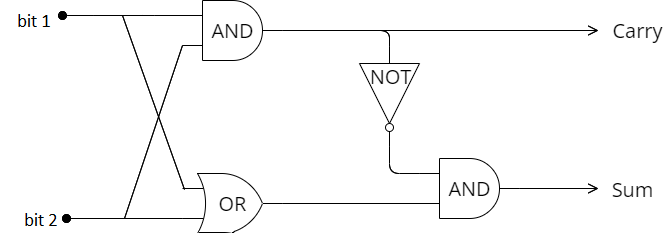
\includegraphics[width=0.5\textwidth]{files/half-adder.png}
    \end{center}
    \begin{enumerate}[(a)]
            \item Formalizujte tento obvod ve výrokové logice. Konkrétně, vyjádřete jej jako teorii $T=\{c\leftrightarrow \varphi,\ s\leftrightarrow \psi\}$ v jazyce $\mathbb P=\{b_1,b_2,c,s\}$, kde výrokové proměnné znamenají po řadě ``bit 1'', ``bit 2'', ``carry'' a ``sum'', a formule $\varphi,\psi$ neobsahují proměnné $c,s$.
            %\item Axiomatizujte teorii $T$ výrokem v CNF a také výrokem v DNF
            \item Dokažte tablo metodou, že $T\models c\to\neg s$.
            %\item Dokažte totéž rezoluční metodou (připomeňte si ji).
    \end{enumerate}

\end{problem}


\begin{problem}

    Pomocí věty o kompaktnosti dokažte, že každý spočetný rovinný graf je obarvitelný čtyřmi barvami. Můžete využít Větu o čtyřech barvách (pro konečné grafy).

\end{problem}

        
\section*{K zamyšlení}
        
        
\begin{problem}

    Dokažte přímo (transformací tabel) \emph{větu o dedukci}, tj. že pro každou teorii $T$ a výroky $\varphi$, $\psi$ platí:
    $$
    T \proves \varphi\to\psi\text{\ \ právě když\ \ }T,\varphi\proves  \psi
    $$

\end{problem}


\begin{problem}
    Mějme dvě neprázdné teorie $A, B$ v témž jazyce. Nechť platí, že každý model teorie $A$ splňuje alespoň jeden axiom teorie $B$. Ukažte, že existují konečné množiny axiomů $\{\alpha_1,\dots,\alpha_k\}\subseteq A$ a $\{\beta_1,\dots,\beta_n\}\subseteq B$ takové, že $\alpha_1\wedge\dots\wedge\alpha_k\,\to\,\beta_1\vee\dots\vee\beta_n$ je tautologie.
\end{problem}
